\documentclass{article}

\usepackage{geometry}
\usepackage{longtable}
\usepackage[dvipsnames,table]{xcolor}
\usepackage{fancyhdr}
\usepackage{xcolor}
\usepackage{graphicx}
\usepackage{hyperref}
\usepackage{float}
\usepackage{listings}
\usepackage{amssymb}
\usepackage{amsmath}
\usepackage{enumitem}
\usepackage{parskip}

% Choose paper size
\geometry{letterpaper, top=25.4mm, bottom=25.4mm, left=25.4mm, right=25.4mm}
%\geometry{a4paper, top=25.4mm, bottom=25.4mm, left=25.4mm, right=25.4mm}

\color{black}
\fancyhf{}
\renewcommand{\headrulewidth}{1pt}
\renewcommand{\footrulewidth}{1pt}

% Define standard IPF color palette
\definecolor{soft-sky-blue}{HTML}{B7DAEB}
\definecolor{orange}{HTML}{FF6633}
\definecolor{cool-grey}{HTML}{91A1B0}
\definecolor{black}{HTML}{000000}
\definecolor{space-blue}{HTML}{003366}
\definecolor{pigeon-blue}{HTML}{5F8396}
\definecolor{sage-green}{HTML}{95A077}
\definecolor{fire-yellow}{HTML}{F9A651}
\definecolor{apple-red}{HTML}{CC4200}
\definecolor{crockadile-green}{HTML}{718944}
\definecolor{slate-grey}{HTML}{607587}
\definecolor{fog-grey}{HTML}{E5E6E9}

% Define certification colors
\definecolor{cert-level-0}{HTML}{CC4200} % apple-red
\definecolor{cert-level-1}{HTML}{FF6633} % orange
\definecolor{cert-level-2}{HTML}{F9A651} % fire-yellow
\definecolor{cert-level-3}{HTML}{B7DAEB} % soft-sky-blue
\definecolor{cert-level-4}{HTML}{5F8396} % pigeon-blue
\definecolor{cert-level-5}{HTML}{718944} % sage-green

\hypersetup{hidelinks}
\pagestyle{fancy}
\pagenumbering{arabic}

\title{

\includegraphics[width=8cm] {images/Rocksavage_Tech_RGB_300.png}\vspace{50pt}
\vspace{10pt} \\
\textbf{DynamicFifo \\
  Product User Guide} \\
{\small{\textcolor{slate-grey}{rocksavagetech.chiselWare.DynamicFifo}}} \\
\vspace{20pt} IPF certified to level:
\textbf{\textcolor{cert-level-0}{0} }of 5 \\
\vspace{5pt}
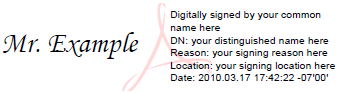
\includegraphics[width=4cm] {images/cert.png}
}

\author{Warren Savage}

\fancyhead[L]{DynamicFifo Users Guide}
\fancyhead[R]{\leftmark}
\fancyfoot[C]{Rocksavage Technology, Inc.\copyright}
\fancyfoot[R]{Page \thepage}

\begin{document}

\maketitle
\newpage
\tableofcontents

\section{Errata and Known Issues}

\subsection{Errata}
\begin{itemize}
      \item{
            Care should be taken in creating instances of \textbf{DynamicFifo}
            with internal very large memory (hundreds or thousands of memory
            cells) as this can generate very large designs. There is currently
            no checks or constraints on users from doing this.
            }

      \item{
            Care should be taken regarding dynamically changing the values on
            the \textit{almostEmptyLevel} and \textit{almostFullLevel} ports
            when the FIFO is not empty as that may result in unpredictable
            behaviors on the \textit{almostEmpty} and \textit{almostFull} flags.
            }
\end{itemize}

\subsection{Known Issues}
None.

% chktex-file 44
\section{Port Descriptions}

The ports for \textbf{DynamicFifo} are shown below in 
Table\ref{table:ports}. The width of several ports is controlled 
by the following input parameters:

\begin{itemize}[noitemsep]
  \item \textit{dataWidth} is the width the dataIn and dataOut ports in bits
  \item \textit{fifoDepth} controls the width of the external RAM addresses
  \item \textit{externalRam} controls whether the ports (below, in gray) are 
    generated for an external dual-port SRAM
\end{itemize}
 
\renewcommand*{\arraystretch}{1.4}
\begin{longtable}[H]{
  | p{0.20\textwidth}
  | p{0.20\textwidth}
  | p{0.12\textwidth}
  | p{0.43\textwidth} |
  }
  \hline
  \textbf{Port Name} &   
  \textbf{Width} &   
  \textbf{Direction} &   
  \textbf{Description} \\ \hline \hline

  clock &       
  1 &       
  Input &       
  Positive edge clock \\ \hline

  reset &       
  1 &       
  Input &       
  Active high reset \\ \hline

  push &       
  1 &       
  Input &       
  Push a word into the FIFO \\ \hline

  pop &        
  1 &       
  Input &       
  Pop a word from the FIFO \\ \hline

  dataIn &      
  \textit{dataWidth} & 
  Input &     
  Data to be pushed into the FIFO \\ \hline

  dataOut &     
  \textit{dataWidth} & 
  Output &    
  Data popped from the FIFO \\ \hline

  empty &       
  1 &       
  Output &      
  Indicates the FIFO is empty \\ \hline

  full &        
  1 &       
  Output &      
  Indicates the FIFO is full \\ \hline

  almostEmptyLevel & 
  log2Ceil(\textit{fifoDepth}) & %chktex 36 
  Input &       
  Sets the threshold for the almostEmpty port.\ almostEmpty will be active 
  when the FIFO is at or below this level.\\ \hline

  almostFullLevel & 
  log2Ceil(\textit{fifoDepth}) & %chktex 36 
  Input &        
  Sets the threshold for the almostFull port.\ almostFull will be active 
  when the FIFO is at or above this level.\\ \hline

  \rowcolor{fog-grey}
  ramWriteEnable &     
  1 &      
  Output &        
  Write enable to the external FIFO RAM \\ \hline
 
  \rowcolor{fog-grey}
  ramWriteAddress & 
  log2Ceil(\textit{fifoDepth}) & %chktex 36 
  Output &    
  Write address to the external FIFO RAM \\ \hline

  \rowcolor{fog-grey}
  ramDataIn &    
  \textit{dataWidth} & 
  Output &    
  Data to the external FIFO RAM \\ \hline
 
  \rowcolor{fog-grey}
  ramReadEnable &
  1 &      
  Input &        
  Read enable to the external FIFO RAM \\ \hline
 
  \rowcolor{fog-grey}
  ramReadAddress & 
  log2Ceil(\textit{fifoDepth}) & %chktex 36 
  Output &    
  Read address to the external FIFO RAM \\ \hline
 
  \rowcolor{fog-grey}
  ramDataOut &   
  \textit{dataWidth} & 
  Input &     
  Data from the external FIFO RAM \\ \hline
 
  \caption{Port Descriptions}\label{table:ports}
\end{longtable}

% chktex-file 44

\section{Parameter Descriptions}

The parameters for \textbf{DynamicFifo} are shown below in
Table~\ref{table:params}.

\renewcommand*{\arraystretch}{1.4}
\begin{longtable}[H]{
    | p{0.25\textwidth}
    | p{0.10\textwidth}
    | p{0.05\textwidth}
    | p{0.05\textwidth}
    | p{0.47\textwidth} |
  }
  \hline
  \textbf{Name} &
  \textbf{Type} &
  \textbf{Min}  &
  \textbf{Max}  &
  \textbf{Description}            \\ \hline \hline

  externalRam   &
  Boolean       &
  false         &
  true          &
  Determines whether to build FIFO memory with flip-flops or provide and
  an external interface to a SRAM \\ \hline

  dataWidth     &
  Int           &
  1             &
  $\ge$ 1       &
  The data width of the FIFO      \\ \hline

  fifoDepth     &
  Int           &
  2             &
  $\ge$ 2       &
  The depth of the FIRO           \\ \hline

  \caption{Parameter Descriptions}\label{table:params}
\end{longtable}

The DynamicFifo is instantiated into a design as follows:

\begin{lstlisting}[language=Scala]

  // Instantiate small FIFO using internal flip-flops
  val mySmallFifo = new DynamicFifo(
    externalRAM = false, 
    dataWidth = 8, 
    fifoDepth = 16) 

  // Instantiate large FIFO using external SRAM
  val myLargeFifo = new DynamicFifo(
    externalRAM = true, 
    dataWidth = 32, 
    fifoDepth = 512) 

  \end{lstlisting}
\section{Theory of Operations}

\subsection{Introduction}
The \textbf{DynamicFifo} is a highly parameterized FIFO and FIFO controller. It
is configurable as a full self-contained FIFO with internal memory being
constructed from flip-flops, or a FIFO controller that uses an external SRAM
for memory.

\begin{figure}[h]
  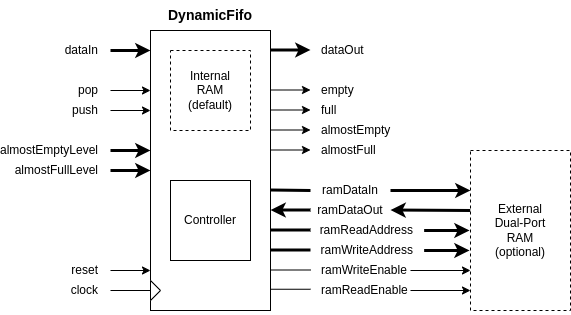
\includegraphics[width=0.80\textwidth]{images/block-diagram.png}
  \caption{Block Diagram}\label{fig:block-diagram}
\end{figure}

It features the following status flags which are described in
Table~\ref{table:ports}.

\begin{itemize}[noitemsep]
  \item{empty}
  \item{full}
  \item{almostEmpty}
  \item{almostFull}
\end{itemize}

When \textit{push} is asserted, the data on the \textit{dataIn} port is enqued
on the next rising edge of \textit{clock}. When \textit{pop} is asserted, the
top of the FIFO is dequed and immediately available on the \textit{dataOut}
port. Pop and Push operations can be simulataneous.

There are two error conditions which produce the following effects:
\begin{itemize}
  \item{When \textit{pop} is asserted and the FIFO is empty (\textit{empty} is
        active), \textit{dataOut} will contain the last valid data held in
        the FIFO.}
  \item{When \textit{push} is asserted and the FIFO is full (\textit{full} is
        active), \textit{dataIn} will be ignored and not enqued.}
\end{itemize}

The \textit{almostEmpty} and \textit{almostFull} flags allow for additional
feedback to the system that is useful for optimizing data flow control. The
levels of these flags can be programmed dynamically through the
\textit{almostEmptyLevel} and \textit{almostFullLevel} ports.

\newpage
\subsection{Interface Timing}

DynamicFifo has a simple, synchronous interface. The timing diagram shown below
in Figure~\ref{fig:timing} represents an instantiation with the following
parameters.

\begin{lstlisting}[language=Scala]
val myFifo = new DynamicFifo(
  externalRAM = true, 
  dataWidth = 16, 
  fifoDepth = 5) 
\end{lstlisting}

\begin{figure}[h]
  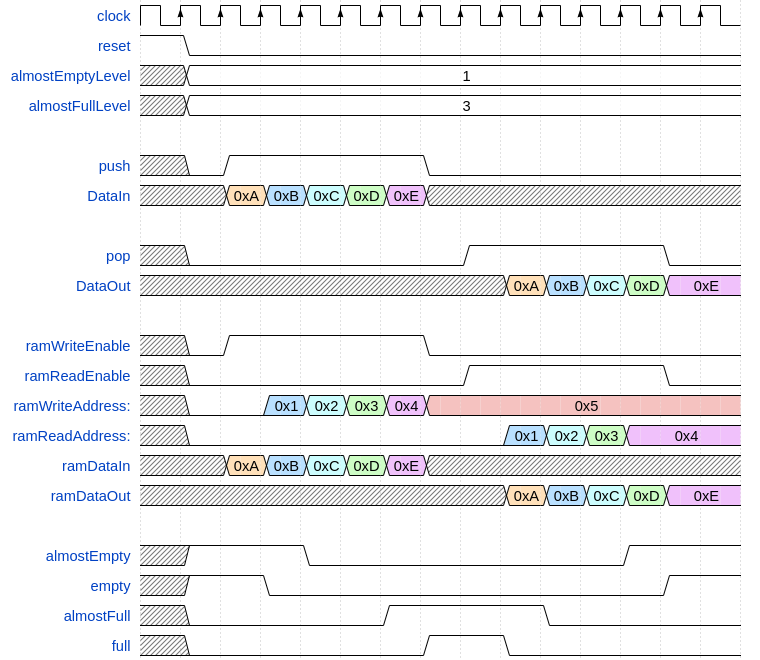
\includegraphics[width=\textwidth]{images/timing.png}
  \caption{Timing Diagram}\label{fig:timing}
\end{figure}

The \textit{almostEmptyLevel} port is driven by external logic to a static value
of 1 after reset and the \textit{almostFull} port is driven to 3.

Beginning in the third clock cycle, 5 words of data are pushed into the
FIFO.\ The status flags show the FIFO going from empty to full.

The FIFO is then fully emptied when the \textit{pop} port is help high for
5 clock cycles. The status flags show the FIFO going from full to empty again.
\section{Simulation}

This section is under construction and will be completed as the code is
completed. But will include the following subsections:

\begin{itemize}
  \item How to configure test operations
  \item How to run tests
  \item List of tests with description of each test
  \item Code coverage results
\end{itemize}
% chktex-file 44
\section{Synthesis}

\subsection{Area}

The DynamicFifo has been tested in a number of configurations and the following
results should be representative of what a user should see in their own
technology.

\renewcommand*{\arraystretch}{1.4}
\begin{longtable}[H]{
    | p{0.20\textwidth}
    | p{0.15\textwidth}
    | p{0.15\textwidth}
    | p{0.15\textwidth}
    | p{0.15\textwidth} |
  }
  \hline
  \textbf{Config Name}   &
  \textbf{externalRAM}   &
  \textbf{dataWidth}     &
  \textbf{fifoDepth}     &
  \textbf{Gates}           \\ \hline \hline

  small\_false\_8\_8     &
  false                  &
  8                      &
  8                      &
  769                      \\ \hline

  medium\_false\_32\_64  &
  false                  &
  32                     &
  64                     &
  19,283                   \\ \hline

  large\_false\_64\_256  &
  false                  &
  64                     &
  256                    &
  152,808                  \\ \hline

  small\_true\_64\_256   &
  true                   &
  64                     &
  256                    &
  355                      \\ \hline

  medium\_true\_128\_128 &
  true                   &
  128                    &
  128                    &
  477                      \\ \hline

  large\_true\_256\_2048 &
  true                   &
  256                    &
  2048                   &
  502                      \\ \hline
  \caption{Synthesis results}\label{table:area}
\end{longtable}

\subsection{SDC File}
An \texttt{.sdc} file is used to provide synthesis and static timing analysis
tools guidance for synthesis.

A \texttt{DynamicFifo.sdc} file is generated for each configuration of
the SystemVerilog code that is emitted and is found in the
\texttt{./generated/<config~name>} directory.

\subsection{Timing}

The following timing was extracted using the generated~.sdc files using the
Nangate 45nm free library.

\renewcommand*{\arraystretch}{1.4}
\begin{longtable}[H]{
    | p{0.20\textwidth}
    | p{0.08\textwidth}
    | p{0.12\textwidth}
    | p{0.13\textwidth}
    | p{0.15\textwidth}
    | p{0.15\textwidth} |
  }
  \hline
  \textbf{Config Name}   &
  \textbf{Period}        &
  \textbf{Duty Cycle}    &
  \textbf{Input Delay}   &
  \textbf{Output Delay}  &
  \textbf{Slack}           \\ \hline \hline

  small\_false\_8\_8     &
  5ns                    &
  50\%                   &
  20\%                   &
  20\%                   &
  4.53 (MET)               \\ \hline

  medium\_false\_32\_64  &
  5ns                    &
  50\%                   &
  20\%                   &
  20\%                   &
  4.29 (MET)               \\ \hline

  large\_false\_64\_256  &
  5ns                    &
  50\%                   &
  20\%                   &
  20\%                   &
  4.40 (MET)               \\ \hline

  small\_true\_64\_256   &
  5ns                    &
  50\%                   &
  20\%                   &
  20\%                   &
  4.40 (MET)               \\ \hline

  medium\_true\_128\_128 &
  5ns                    &
  50\%                   &
  20\%                   &
  20\%                   &
  4.30 (MET)               \\ \hline

  large\_true\_256\_2048 &
  5ns                    &
  50\%                   &
  20\%                   &
  20\%                   &
  4.37 (MET)               \\ \hline
  \caption{Staic Timing Analysis results}\label{table:timing}
\end{longtable}

\subsection{Multicycle Paths}
None.


\end{document}
